% (c) 2015 Daniele Zambelli daniele.zambelli@gmail.com
% (c) 2016 Andrea Sellaroli andrea.sellaroli@istruzione.it

\chapter{Calcolo combinatorio}

\section{Il calcolo combinatorio}
\label{sec:01_introduzione}
Capita spesso di dover scegliere degli elementi da un insieme finito e di 
doverli ordinare in una sequenza. Uno dei problemi principali che si pone è 
\emph{contare} in quanti modi si possono disporre questi oggetti. Ad esempio, 
quante password di 6 caratteri posso ottenere? Quanti anagrammi della parola 
"MATEMATICA" posso fare? Quante sono le possibili colonne del totocalcio?

Iniziamo ad affrontare questi problemi con una situazione abbastanza semplice. 
Tre studenti, Alice, Barbara e Carlo, devono decidere in che ordine presentarsi 
ad un'interrogazione programmata.
In quanti modi possibili possono organizzarsi?
Proviamo a visualizzare la cosa. Il primo studente può essere scelto 
all'interno dell'insieme $\{Alice,Barbara,Carlo\}$, che contiene 3 elementi. Nel 
diagramma seguente per ogni ramo dell'albero abbiamo rappresentato una delle 
possibili scelte del primo studente ad essere interrogato.

\vspace{-6pt}
\begin{center}
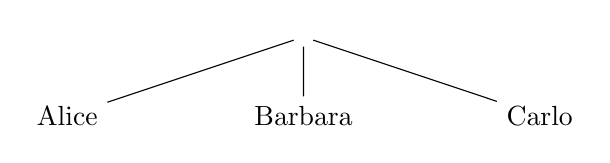
\begin{tikzpicture}[level distance=1.0cm,
  level 1/.style={sibling distance=3cm},
  level 2/.style={sibling distance=1.5cm}]


  \node {}
    child {node {Alice}}
    child {node {Barbara}}
	child {node {Carlo}};

\end{tikzpicture}
\end{center}

\vspace{-6pt}
Per scegliere chi verrà interrogato per secondo dobbiamo invece tenere conto di 
chi è già stato interrogato per primo. Ad, esempio, se il primo ad essere 
scelto è stato $Carlo$, l'insieme da cui potrò scegliere è $\{Alice, Barbara\}$ 
che è formato da due soli elementi. Il diagramma ad albero ci permette di dare 
una comoda rappresentazione. Per ognuno dei tre rami precedenti costruiamo due 
nuovi rami che contengono i due studenti che non sono stati interrogati per 
primi.

\vspace{-12pt}
\begin{center}
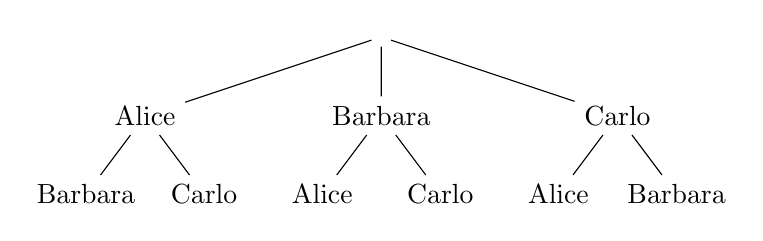
\begin{tikzpicture}[level distance=1.0cm,
  level 1/.style={sibling distance=3cm},
  level 2/.style={sibling distance=1.5cm}]


  \node {}
    child {node {Alice}
      child {node {Barbara}}
      child {node {Carlo}}
    }
    child {node {Barbara}
    child {node {Alice}}
      child {node {Carlo}}
    }
	child {node {Carlo}
      child {node {Alice}}
      child {node {Barbara}}
    };

\end{tikzpicture}
\end{center}

\vspace{-12pt}
La scelta del terzo studente ad essere interrogato è obbligata. Infatti se i 
primi due ad essere interrogati sono stati Barbara e Carlo, necessariamente 
adesso sarà la volta di Alice. L'albero completo si presenta così:

\vspace{-12pt}
\begin{center}
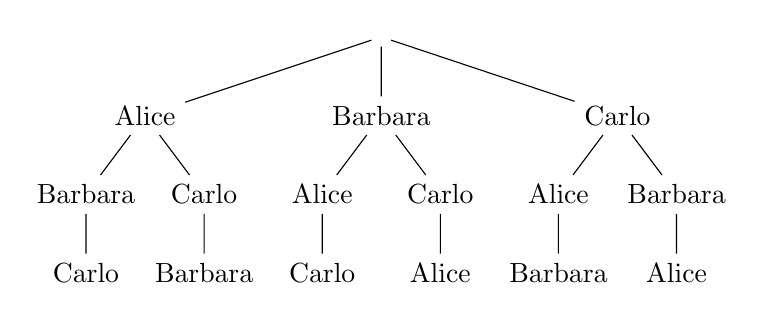
\begin{tikzpicture}[level distance=1.0cm,
  level 1/.style={sibling distance=3cm},
  level 2/.style={sibling distance=1.5cm}]


  \node {}
    child {node {Alice}
      child {node {Barbara} child {node {Carlo}}}
      child {node {Carlo} child {node {Barbara}}}
    }
    child {node {Barbara}
    child {node {Alice} child {node {Carlo}}}
      child {node {Carlo} child {node {Alice}}}
    }
	child {node {Carlo}
      child {node {Alice} child {node {Barbara}}}
      child {node {Barbara} child {node {Alice}}}
    };

\end{tikzpicture}
\end{center}

Ognuno dei possibili ordinamenti è adesso rappresentato in un percorso che va 
dalla radice dell'albero fino ad un nodo terminale. In totale i possibili 
ordinamenti sono quindi 6 ovvero

\begin{tabular}{ccc}
	$Alice, Barbara, Carlo$ & $Barbara, Alice, Carlo$ & $Carlo, Alice, 
Barbara$\\
	$Alice, Carlo, Barbara$ & $Barbara, Carlo,Alice$ & $Carlo, Barbara, 
Alice$\\
\end{tabular}

\vspace{.2cm}
Un altro modo di vedere la cosa è il seguente. Immaginiamo di avere tre scatole 
vuote che rappresentano le tre posizioni in cui possono essere interrogati i 
tre studenti.

\begin{center}
\begin{tabular}{ccc}
\fbox{\phantom{3}} & \fbox{\phantom{2}} & \fbox{\phantom{1}}\\

\end{tabular}
\end{center}

Il primo studente può essere scelto in 3 modi diversi. La scelta del secondo 
dipenderà dal primo e quindi potrà essere scelto solo tra due possibilità. La 
scelta del terzo studente invece è obbligata, che equivale a dire che può 
essere scelto solo in un modo.

\begin{center}
\begin{tabular}{ccc}
\fbox{3} & \fbox{2} & \fbox{1}\\

\end{tabular}
\end{center}

Questo significa che per ognuna delle tre scelte del primo studente è possibile 
fare due scelte del secondo e una del primo. L'operazione matematica che ci 
permette di determinare in quanti modi si possono ordinare 3 studenti è quindi 
la moltiplicazione. In questo caso gli studenti possono essere interrogati in 
$6 = 3 \cdot 2 \cdot 1$ modi diversi. La generalizzazione di questa idea prende 
il nome di \emph{principio di moltiplicazione}. Se una scelta può essere fatta 
in $n_1$ modi diversi, e per ciascuno di questi modi una seconda scelta può 
essere fatta in $n_2$ modi diversi e per ognuno dei modi in cui sono fatte le 
due prime scelte una terza scelta può essere fatta in $n_3$ modi diversi e così 
via per $k$ scelte, allora il numero totale di scelte è $n_1 \cdot n_2 \cdot n_3 
\cdot ... \cdot n_k$.
\begin{exrig}
\begin{esempio}
In un armadio ci sono 6 magliette, 4 paia di pantaloni, 2 cappelli e 3 paia di 
scarpe. In quanti modi diversi è possibile vestirsi?

Costruiamo quattro caselle che corrispondono ai quattro capi di abbigliamento 
del problema. La prima casella, ad esempio, è quella relativa alle magliette 
che possono essere scelte in 6 modi diversi; la seconda è quella dei pantaloni, 
che possono essere scelti in 4 modi diversi
\begin{center}
\begin{tabular}{cccc}
\fbox{6} & \fbox{4} & \fbox{2} & \fbox{3}\\

\end{tabular}
\end{center}
Il numero totale dei modi in cui è possibile vestirsi è quindi $6 \cdot 4 \cdot 
2 \cdot 3 = 144$. Poiché la moltiplicazione è commutativa, è interessante 
notare che l'ordine in cui vengono scelti gli indumenti non è importante. Se 
prima scegliessi il cappello e poi i pantaloni il risultato sarebbe lo stesso.
\end{esempio}
\end{exrig}

Analizzeremo nel seguito diversi casi che si presentano con una certa frequenza 
e che possono essere risolti utilizzando il principio di moltiplicazione.




%Nell'esempio che abbiamo appena visto sarebbe considerata una grande 
ingiustizia se il nome di uno studente comparisse due volte nell'elenco. In 
questo caso di dice che tale problema è \emph{senza ripetizioni}. In molte 
situazioni però è normale che gli elementi possano essere ripetuti, basta 
pensare che per formare un numero di telefono non c'è alcun problema se alcune 
cifre compaiono più volte. Nei prossimi paragrafi analizzeremo tutte le 
casistiche che si possono presentare.


\section{Permutazioni}
\label{sec:02_permutazioni}
Abbiamo visto che per ordinare 3 studenti sono possibili 6 modi distinti. E se 
gli studenti fossero 10? Applicando il ragionamento precedente il primo 
studente lo posso scegliere in 10 modi diversi, il secondo solo in 9 modi 
diversi visto che il primo è già stato scelto e così via.

\begin{center}
\begin{tabular}{cccccccccc}
\fbox{10} & \fbox{9} & \fbox{8} & \fbox{7} & \fbox{6} & \fbox{5} & \fbox{4} & 
\fbox{3} & \fbox{2} & \fbox{1}\\
\end{tabular}
\end{center}

Applicando il principio di moltiplicazione il numero degli ordinamenti 
possibili è quindi $10\cdot 9\cdot 8\cdot 7\cdot 6\cdot 5\cdot 4\cdot 3\cdot 
2\cdot 1 = 3628800$. 

Questo prodotto ha per fattori tutti i numeri naturali da 1 a 10. \`{E} un 
importante operazione matematica che prende il nome di fattoriale. 
\begin{definizione}
Il \emph{fattoriale} di un numero naturale $n$, indicato con $n!$, è il 
prodotto dei numeri interi positivi minori o uguali ad $n$, ovvero $$n!=n\cdot 
(n-1) \cdot (n-2) \cdot ... \cdot 3 \cdot 2 \cdot1$$ Per convenzione $0! = 1$.
\end{definizione}

Ad esempio $10!=3628800$. A questo punto possiamo generalizzare facilmente al 
caso generico di un insieme formato da $n$ elementi. 

\begin{definizione}
Le \emph{permutazioni} di $n$ elementi sono tutti i possibili allineamenti che 
si ottengo scambiando di posto $n$ oggetti; il numero delle permutazioni è
$$n!$$
\end{definizione}
\begin{exrig}
\begin{esempio}
Quanti sono i possibili anagrammi, anche senza senso, della parola VERONA?
L'insieme delle lettere $\{V,E,R,O,N,A\}$ è formato da 6 elementi e quindi 
tutti i possibili anagrammi sono $6!=720$.
\end{esempio}
\end{exrig}

Nell'esempio precedente abbiamo potuto usare il \emph{principio della 
moltiplicazione} perché le lettere che formano la parola VERONA sono tutte 
diverse. Nel caso in cui una lettera venga ripetuta più volte la situazione è 
più complessa.
Proviamo ad analizzare tutti i possibili anagrammi della parola MAMMA: in 
questo caso compaiono 3 volte la lettera M e 2 volte le lettere A. Per calcolare 
il numero di possibili anagrammi ragioniamo nel modo seguente. Mettiamo un 
indice alle lettere uguali per distinguerle:
$$M_1 A_1 M_2 M_3 A_2$$.
Se calcolo tutte le possibili permutazioni risulta $5!=120$. Tuttavia le due 
permutazioni $M_1 M_2 M_3 A_1 A_2$ e $M_1 M_2 M_3 A_2 A_1$ rappresentano la 
stessa parola MMMAA. Le 120 permutazioni che si ottengono se le lettere sono 
distinguibili va quindi diviso per le possibili permutazioni della lettera A 
che sono $2!$. Lo stesso ragionamento si può ripetere per la lettera M, in 
questo caso le permutazioni sono $3!=6$. In definitiva tutti gli anagrammi della 
parola MAMMA sono
$\dfrac{6!}{2!\cdot 3!}=10$.

\begin{definizione}
Le \emph{permutazioni} di $n$ elementi di cui $k_1$ uguali tra loro, $k_2$ 
uguali tra loro e distinti dai precedenti, ... $k_p$ uguali tra loro e distinti 
dai precedenti, sono:
$$ \dfrac{n!}{k_1!\cdot k_2! \cdot ... \cdot k_p!}$$
\end{definizione}

\begin{esempio}
Quanti sono i possibili anagrammi della parola MATEMATICA?
Le lettere che formano la parola MATEMATICA sono 10. La lettera A è ripetuta 3 
volte, le lettere M e T sono ripetute 2 volte. I possibili anagrammi quindi sono
$\dfrac{10!}{3!\cdot 2!\cdot 2!}=151200$
\end{esempio}


\section{Disposizioni}
\label{sec:03_disposizioni}
Nelle permutazioni il numero di elementi ed il numero di posti è uguale. In 
alcune situazioni può capitare che il numero dei posti sia inferiore al numero 
di elementi. 
Ad esempio, vogliamo calcolare quante sono le parole di tre lettere, anche 
senza significato, che si possono formare usando le 26 lettere dell'alfabeto 
italiano senza che ci siano lettere ripetute. Come per i casi precedenti, la 
prima lettera può essere scelta in 26 modi diversi, la seconda solo in 25 e la 
quarta in 24 modi:
\begin{center}
\begin{tabular}{ccc}
\fbox{26} & \fbox{25} & \fbox{24}\\
\end{tabular}
\end{center}

Il risultato è che le possibili parole di 3 lettere in modo che non compaiano 
lettere ripetute è $26 \cdot 25 \cdot 24 = 15600$.

Si può riscrivere questo calcolo usando il fattoriale in una forma che ci sarà 
utile per il seguito. Infatti $$26 \cdot 25 \cdot 24 =\dfrac{26 \cdot 25 \cdot 
24 \cdot \cancel{23} \cdot \cancel{22} \cdot ... \cdot 
\cancel{2}\cdot\cancel{1}}{\cancel{23} \cdot \cancel{22} \cdot ... \cdot 
\cancel{2}\cdot\cancel{1}} = \dfrac{26!}{23!}=\dfrac{26!}{(26-3)!}$$

\begin{definizione}
Le \emph{disposizioni} di $n$ elementi in $k$ posti, con $n\geq k$, sono tutte 
le scelte ordinate di $k$ elementi tra gli $n$ disponibili. 


Il numero delle disposizioni è
$$\underbrace{n\cdot (n-1) \cdot (n-2) \cdot ... \cdot (n-k+1)}_{\text{k 
volte}}=\dfrac{n!}{(n-k)!}$$
\end{definizione}

\begin{esempio}
In un gruppo di 19 studenti, in quanti modi possono scelti 4 studenti per 
essere interrogati?
In questo caso abbiamo $19$ elementi per $4$ posti, quindi il numero delle 
possibili disposizioni è
$19\cdot 18 \cdot 17 \cdot 16 = \dfrac{19!}{(19-4)!}= \dfrac{19!}{15!} = 93024$.

\end{esempio}

\section{Combinazioni}
\label{sec:04_combinazioni}
Esaminiamo i seguenti problemi, all'apparenza molto simili
\begin{itemize} [nosep]
\item Da un insieme di 10 studenti ne devono essere selezionati 4 per essere 
interrogati in 4 giorni distinti.
\item Da un insieme di 10 studenti ne devono essere selezionati 4 per essere 
interrogati lo stesso giorno.
\end{itemize}
In entrambi i problemi abbiamo $n=10$ elementi da distribuirsi in $k=4$ posti. 
Nel primo caso, tuttavia, l'ordine è importante, mentre nel secondo 
è indifferente in che sequenza vengono scelti.
La soluzione del primo caso è una \emph{disposizione}, come visto nel paragrafo 
precedente, e quindi risulta:
$$\dfrac{10!}{(10-4)!}=\dfrac{10!}{6!}=5040$$

Se gli studenti vengono interrogati contemporaneamente non ha alcuna importanza 
in che ordine vengono scelti. 
Tra le $5040$ possibilità precedenti ce ne sono ovviamente molte di uguali. Se 
indichiamo con A,B,C e D ognuna dei seguenti ordini è conteggiato nei $5040$:
\begin{center}
\begin{tabular}{cccccc}
$A B C D$ & $A B D C$ & $A C B D$ & $A C D B$ & $A D B C $ & $A D C B$\\
$B A C D$ & $B A D C$ & $B C A D$ & $B C D A$ & $B D A C $ & $B D C A$\\
$C A B D$ & $C A D B$ & $C B A D$ & $C B D A$ & $C D A B $ & $C D B A$\\
$D A C B$ & $D A B C$ & $D C A B$ & $D C B A$ & $D B A C $ & $D B C A$\\
\end{tabular}
\end{center}
In totale fanno $24$ ordini possibili che è il numero di permutazioni di 4 
elementi, infatti $4!=24$. Questa situazione si ripete uguale per ogni 
possibile scelta dei quattro elementi tra i 10. Se non siamo interessati 
all'ordine quindi possiamo quindi dividere il numero di disposizioni di 10 
elementi in 4 posti per il numero di permutazioni di permutazioni di 4 elementi.

$$\dfrac{10!}{(10-4)!}\cdot\dfrac{1}{4!}=\dfrac{10!}{6!4!}=210$$


\begin{definizione}
Le \emph{combinazioni} di $n$ elementi di classe $k$ sono ognuna delle scelte 
di $k$ elementi tra gli $n$ senza che conti l'ordine in cui sono scelti. Il 
numero delle combinazioni è
$$ \dfrac{n!}{k!(n-k)!}$$
\end{definizione}
\begin{esempio}
Quante sono le possibili cinquine che si possono fare nella tombola (90 numeri)?

Si tratta delle combinazioni di 90 elementi in 5 posti (infatti non è 
importante l'ordine in cui i numeri vengono estratti per fare cinquina). Le 
possibilità sono quindi:
$$ \dfrac{90!}{(90-5)!5!}=43 949 268$$
\end{esempio}

Vista la grande importanza che rivestono, il numero di combinazioni si indica 
con un simbolo specifico

\begin{definizione}
Il \emph{coefficiente binomiale} è definito come 
$$ \binom{n}{k}=\dfrac{n!}{k!(n-k)!}$$
\end{definizione}



